\chapter{BP File Format}

\section{Introduction}

This chapter describes the file structure of BP, which is the ADIOS native binary 
file format, to aid in understanding ADIOS performance issues and how files convert 
from BP files to other scientific file formats, such as netCDF and HDF5.

To avoid the file size limitation of 2 gigabytes by using a signed 32-bit offset 
within its internal structure, BP format uses an unsigned 64-bit datatype as the 
file offset. Therefore, it is possible to write BP files that exceed 2 gigabytes 
on platforms that have large file support. 

By adapting ADIOS read routines based on the endianness indication in the file 
footer, BP files can be easily portable across different machines (e.g., between 
the Cray-XT4 and BlueGene). 

To aid in data selection, we have a low-overhead concept of data characteristics 
to provide an efficient, inexpensive set of attributes that can be used to identify 
data sets without analyzing large data content.

As shown in Figure \ref{fig:bp-file-struct}, 
the BP format comprises a series of process groups and the 
file footer. The remainder of this chapter describes each component in detail and 
helps the user to better understand (1) why BP is a self -describing and metadata-rich 
file format and (2) why it can achieve high I/O performance on different machine 
infrastructures. 

\begin{figure}[htbp]
\begin{center}
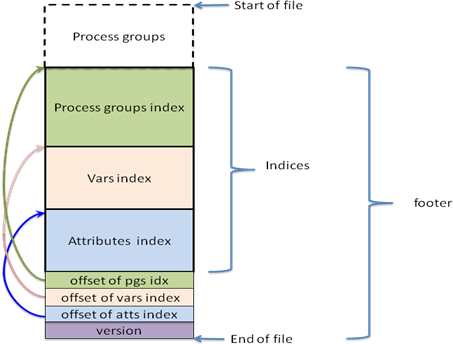
\includegraphics[width=217pt, height=163pt]{figures/bp-file-structure.png}
\caption{BP file structure}
\label{fig:bp-file-struct}
\end{center}
\end{figure}

\section{Footer}

One known limitation of the NetCDF format is that the file contents are stored 
in a header that is exactly big enough for the information provided at file creation. 
Any changes to the length of that data will require moving data. To avoid this 
cost, we choose to employ a foot index instead. We place our version identifier 
and the offset to the beginning of the index as the last few bytes of our file, 
making it simple to find the index information and to add new and different data 
to our files without affecting any data already written. 

\subsection{Version}

We reserve 4 bytes for the file version, in which the highest bit indicates endianness. 
Because ADIOS uses a fixed-size type for data, there is no need to store type size 
information in the footer. 

\subsection{Offsets of indices}

In BP format, we store three 8-byte file offsets right before the version word, 
which allows users or developers to quickly seek any of the index tables for process 
groups, variables, or attributes. 

\subsection{Indices}

\subsubsection{Characteristics}

Before we dive into the structures of the three index tables mentioned earlier, 
let's first take a look what characteristic means in terms of BP file format. To 
be able to make a summary inspection of the data to determine whether it contains 
the feature of greatest interest, we developed the idea of data characteristics. 
The idea of data characteristics is to collect some simple statistical and/or analytical 
data during the output operation or later for use in identifying the desired data 
sets. Simple statistics like array minimum and maximum values can be collected 
without extra overhead as part of the I/O operation. Other more complex analytical 
measures like standard deviations or specialized measures particular to the science 
being performance by require more processing. As part of our BP format, we store 
these values not only as part of data payload, but also in our index. 

\subsubsection{PG Index table}

As shown in Figure \ref{fig:group-index-table}, 
the process group (PG) index table encompasses the count 
and the total length of all the PGs as the first two entries. The rest of the tables 
contain a set of information for each PG, which contains the group name information, 
process ID, and time index. The Process ID specifies which process a group is written 
by. That process will be the rank value in the communicator if the MPI method is 
used. Most importantly, there is a file-offset entry for each PG, allowing a fast 
skip of the file in the unit of the process group.

\begin{figure}[htbp]
\begin{center}
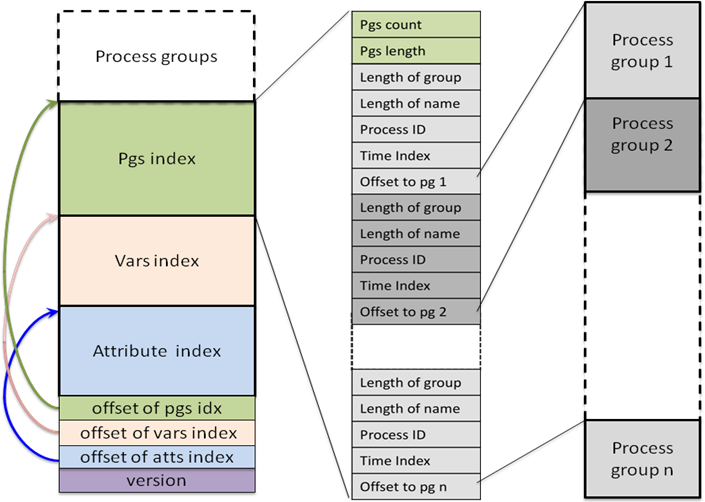
\includegraphics[width=338pt, height=238pt]{figures/group-index-table.png}
\caption{Group index table}
\label{fig:group-index-table}
\end{center}
\end{figure}

\subsubsection{Variables index table}

The variables index table is composed of the total count of variables in the BP 
file, the size of variables index table, and a list of variable records. Each record 
contains the size of the record and the basic metadata to describe the variable. 
As shown in Figure \ref{fig:variables-index-table}, 
the metadata include the name of the variable, the name 
of the group the variable is associated with, the data type of the variable, and 
a series of characteristic features. The structure of each characteristic entry 
contains an offset value, which is addressed to the certain occurrence of the variable 
in the BP file. For instance, if n processes write out the variable ``d'' per time 
step, and m iterations have been completed during the whole simulation, then the 
variable will be written (m\textit{ }\ensuremath{\times} n) times in the BP file 
that is produced. Accordingly, there will be the same number of elements in the 
list of characteristics. In this way, we can quickly retrieve the single dataset 
for all time steps or any other selection of time steps. This flexibility and efficiency 
also apply to a scenario in which a portion of records needs to be collected from 
a certain group of processes. 

\begin{figure}[htbp]
\begin{center}
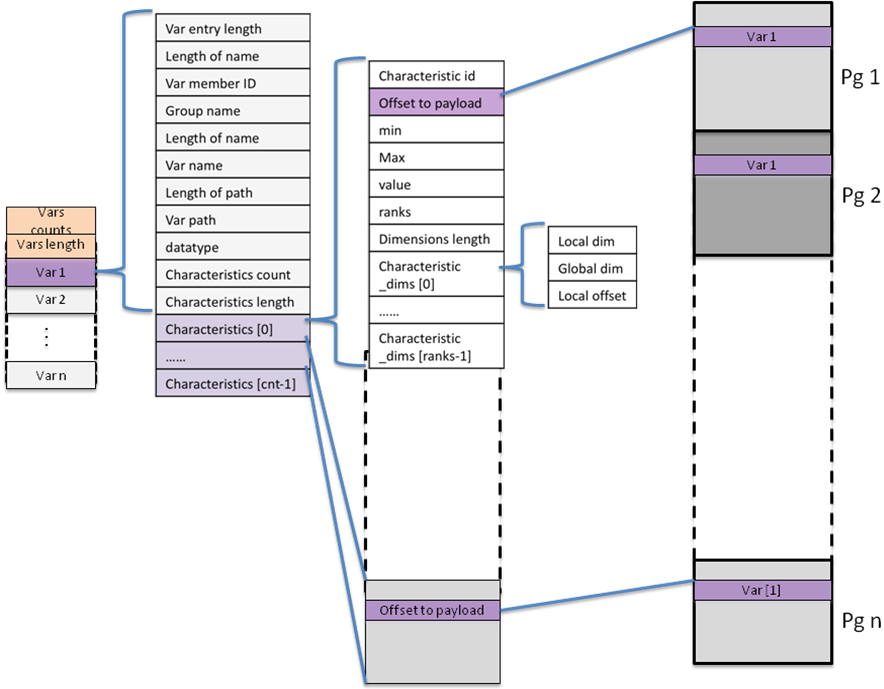
\includegraphics[width=420pt, height=327pt]{figures/variables-index-table.png}
\caption{Variables index table}
\label{fig:variables-index-table}
\end{center}
\end{figure}

\subsubsection{Attributes index table}

Since an attribute can be considered to be a special type of variable, its index 
table in BP format is organized in the same way as a variables index table and 
therefore supports the same types of features mentioned in the previous sections. 

\section{Process Groups}

One of the major concepts in BP format is what is called ``process group'' or PG. 
The BP file format encompasses a series of PG entries and the BP file footer. Each 
process group is the entire self-contained output from a single process and is 
written out independently into a contiguous disk space. In that way, we can enhance 
parallelism and reduce coordination among processes in the same communication group. 
The data diagram in Figure \ref{fig:process-group-struct} 
illustrates the detailed content in each PG. 

\begin{figure}[htbp]
\begin{center}
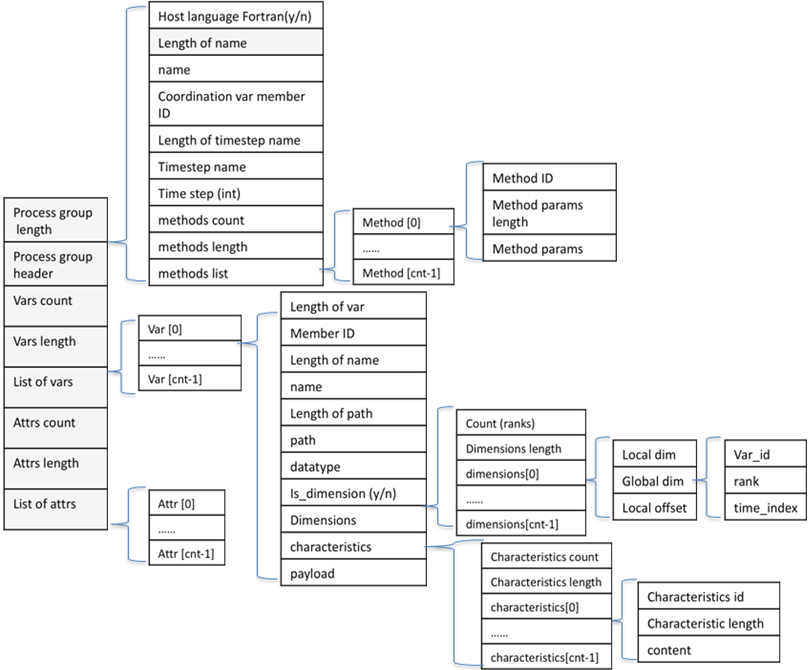
\includegraphics[width=389pt, height=321pt]{figures/process-group-structure.png}
\caption{Process group structure}
\label{fig:process-group-struct}
\end{center}
\end{figure}

\subsection{PG header}

\subsubsection{Unlimited dimension}

BP format allows users to define an unlimited dimension, which will be specified 
as the time-index in the XML file. Users can define variables having a dimension 
with undefined length, for which the variable can grow along that dimension. PG 
is a self-contained, independent data structure; the dataset in the local space 
per each time step is not reconstructed at the writing operations across the processes 
or at time steps. Theoretically, PGs can be appended to infinity; they can be added 
one after another no matter how many processes or time steps take place during 
the simulation.  Thus ADIOS is able to achieve high I/O performance.

\subsubsection{Transport methods}

One of the advantages of organizing output in terms of groups is to categorize 
all the variables based on their I/O patterns and logical relationships. It provides 
flexibility for each group to choose the optimized transport method according to 
the simulation environment and underlying hardware configuration or the transport 
methods used for a performance study without even changing the source code. In 
PG header structure, each entry in the method list has a method ID and method parameters, 
such as system-tuning parameters or underneath driver selection. 

\subsection{Vars list}

\subsubsection{Var header}

\emph{Dimensions structure.} 
Internal to bp is sufficient information to recreate any global structure and to 
place the local data into the structure. In the case of a global array, each process 
writes the size of the global array dimensions, specifies the local offsets into 
each, and then writes the local data, noting the size in each dimension. On conversion 
to another format, such as HDF5, this information is used to create hyperslabs 
for writing the data into the single, contiguous space. Otherwise, it is just read 
back in and used to note where the data came from. In this way, we can enhance 
parallelism and reduce coordination. All of our parallel writes occur independently 
unless the underlying transport specifically requires collective operations. Even 
in those cases, the collective calls are only for a full buffer write (assuming 
the transport was written appropriately) unless there is insufficient buffer space. 

As shown in Figure 19, the dimension structure contains a time index flag, which 
indicates whether this variable has an unlimited time dimension. Var\_id is used 
to retrieve the dimension value if the dimension is defined as variable in the 
XML file; otherwise, the rank value is taken as the array dimension.  

\subsubsection{Payload}

Basic statistical characteristics give users the advantage for quick data inspection 
and analysis. In Figure 19, redundant information about characteristics is stored 
along with variable payload so that if the characteristics part in the file footer 
gets corrupted, it can still be recovered quickly. Currently, only simple statistical 
traits are saved in the file, but the characteristics structure will be easily 
expanded or modified according to the requirements of scientific applications or 
the analysis tools. 

\subsection{Attributes list}

The layout of the attributes list (see Figure \ref{fig:attribute-entry-struct}) 
is very similar to that of the 
variables. However, instead of containing dimensional structures and physical data 
load, the attribute header has an is\_var flag, which indicates either that the 
value of the attribute is referenced from a variable by looking up the var\_id 
in the same group or that it is a static value defined in the XML file. 

\begin{figure}[htbp]
\begin{center}
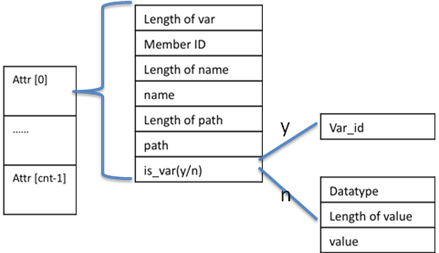
\includegraphics[width=210pt, height=120pt]{figures/attributes-entry-structure.png}
\caption{Attribute entry structure}
\label{fig:attribute-entry-struct}
\end{center}
\end{figure}

